\section{Decomposition 1: SIoTIP System (Av3, UC14, UC15, UC18)}

\subsection{Module to decompose}
    In this run we decompose the \texttt{SIoTIP System}.


\subsection{Selected architectural drivers}
    The non-functional drivers for this decomposition are:
    \begin{itemize}
    	\item \emph{Av3}: Pluggable device or mote failure
    \end{itemize}

    \noindent The related functional drivers are:
    \begin{itemize}
    	\item \emph{UC14}: Send heartbeat (Av3) \\
              This use case checks whether or not motes and pluggable devices
              are still operational.
    	\item \emph{UC15}: Send notification (Av3) \\
              This use case sends a notification to a registered user.
    	\item \emph{UC18}: Check and deactivate applications (Av3) \\
              This use case deactivates any application that requires deactivation,
              because of unavailability of essential pluggable devices
              or unassigned mandatory roles.
    \end{itemize}

    \paragraph{Rationale}
        Av3 was chosen first since it has high priority and it is more relevant to
        the core of the system than the other quality requirements with high
        priority (M1 and U2).
        We believe that handling pluggable device failure/connectivity is
        more important to the whole of the system than M1 and U2, and that
        handling this first would give a stronger starting point for later ADD iterations
        than M1 or U2.


\subsection{Architectural design}\label{sec:architectural-design}
    This section describes what needs to be done to satisfy the requirements for
    this decomposition and how involved problems/obstacles are solved.
    % Detection:
    %     Ping/Echo, Monitor, Heartbeat, Timestamp
    % Resolution:
    %     notifications to 3 stakeholders, degradation/removal from service -> turn off apps

    \paragraph{Av3: Failure detection}
        A SIoTIP gateway can autonomously detect failure of one of its
        connected motes and pluggable devices.
        timers? \\
        heartbeat/timestamp tactic

    \paragraph{Av3: Application deactivation}
        Applications that can no longer operate due to failure of a pluggable
        device or mote should be automatically suspended and re-activated once the failure is resolved.

        Applications need pluggable devices for the proper functioning.
        When the pluggable devices fail, \texttt{the PluggableDeviceManager} sends
        command and \texttt{the ApplicationManager} deactivate one or more applications
        using those devices. Availability and reliability of the shared platform offered to applications is
        important. To reduce the risk of frequent application downtime,
        an application provider can require a redundancy in the available
        pluggable devices. Multiple sensors or actuators for one application can be in one room.
        If one of sensor or actuator failed application just start using
        the other available sensor or actuator in room.

    \paragraph{Av3: Notifications}
        The infrastructure owner should be notified of any persistent pluggable device or mote
        failures. Customer organisations should be notified if one or more of their applications is suspended
        or re-activated. Applications using a failed pluggable device or any device on a failed mote should be
        notified.
        One of the important things for Av3 is notification. In the case
        of failure of sensor, it is mandatory to inform all involved parties
         about the failure to resolve the problem as soon as possible.
        \texttt{The NotificationHandler} notify an infrastructure owner of
        any persistent pluggable device or mote failures. The infrastructure
        owner has to receive the notification in ten seconds in case mote failed or
        in thirty seconds if a pluggable device failed. Notification is also send
        to a customer organisation, when one or more of their application are
        susspended or re-activated. Applications using a failed  pluggable
        device should be also notified via \texttt{The NotificationHandler}.

    \paragraph{Av3: Application redundancy settings}
        Application providers can design their applications such that they explicitly
        require redundancy in the available pluggable devices.

    \subsubsection{Alternatives considered}
        \paragraph{Av3: Alternatives for notifications}
            The notifications are very important part of our system to faster
            solve the problems, when something gets wrong. Our SIoTIP sytem 
            is using external delivery service for sending notifications. 
            Sometimes external services could not be available and it can cuase
            problems. The more our system is dependend on external services the more 
            is our system unreliable. Thus, when we want to offer more reliable 
            platform to our clinets, it is useful to implement our own service
            that can send notifications. This will require adding now enums and tables 
            in \texttt{the Database} and we will implement \texttt{Factory pattern} for this purpose. 
            Each message channel will have its own SendMessage 
            implementation and we can easily add a new message channel with little effort
            in the future. But whole implementation of notification system requires time,
             what we can consider as disadvantage.


\subsection{Instantiation and allocation of functionality}
    This section describes the components which instantiate our solutions described
    in the section above and how the components are deployed on physical nodes.

    \paragraph{Decomposition}
        Figure \ref{fig:it1-cc_main} shows the components resulting from the
        decomposition in this run.

        \begin{figure}[!htp]
        	\centering
        	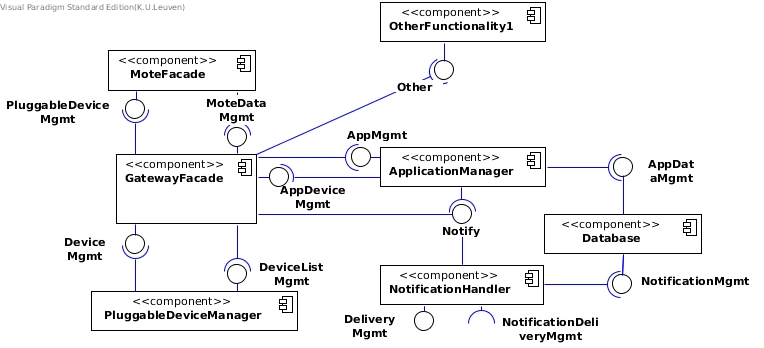
\includegraphics[width=1.00\textwidth]{component-diagram-1}
        	\caption{Component-and-connector diagram of this decomposition.}
            \label{fig:it1-cc_main}
        \end{figure}

        \noindent The responsibilities of the components are as follows:

    \subparagraph{ApplicationManager}
        Responsible for deactivating applications and after this action calls method of
        \texttt{the NotificationHandler} to send notification to a customer organisation.
        When \texttt{the ApplicationManager} detects that application uses failed pluggable devices,
        then the notification is sent to an application.

        set redundancy in the available pluggable devices??
        (Av3) ???? check mandatory user roles

    \subparagraph{Database}
        General database for other data. For instance the Database storages the data
        of notifications (Av3).

    \subparagraph{GatewayFacade}
        Receives heartbeats from pluggable devices and sends heartbeats/device lists.
        \texttt{The GatewayFacade} sends commands to \texttt{the ApplicationManager}
        to shutdown applications, if is it needed. \\

        send notification trigger ???(Av3)\\
        forward data to applications

    \subparagraph{MoteFacade}
        Sends heartbeats from pluggable devices to\texttt{the PluggableDeviceFacade}.

    \subparagraph{NotificationHandler}
        Responsible for send notifications to infrastructure owner, customer organisation
        and applications (Av3). \\
        stored by system \(->\) contact DB? \\
        lookup communication channel \\
        users choose delivery method?

    \subparagraph{PluggableDeviceFacade}
        Sends heartbeats to \texttt{the MoteFacade}.

    \subparagraph{PluggableDeviceManager}
        Checks list of devices and see if there are pluggable devices for applications.
        \texttt{the PluggableDeviceManager} contains application preferences (e.g. amount of sensors required) and
        can send command to deactivate application.
        Send information about new/needed hardware is detected to \texttt{the GatewayFacade}, that sends command to
        reactivate application.
        check redundancy in the available pluggable devices??? is not the same like first sentence???

    % \paragraph{Behaviour}
    % A SEQUENCE DIAGRAM WOULD BE USEFUL FOR
    % UC11: shows how the gateway checks if devices are initialised
    % UC14: shows how applications can get deactivated

    \paragraph{Deployment}
        Figure \ref{fig:it1-depl_main} shows the allocation of components
        to physical nodes.

        \begin{figure}[!htp]
        	\centering
        	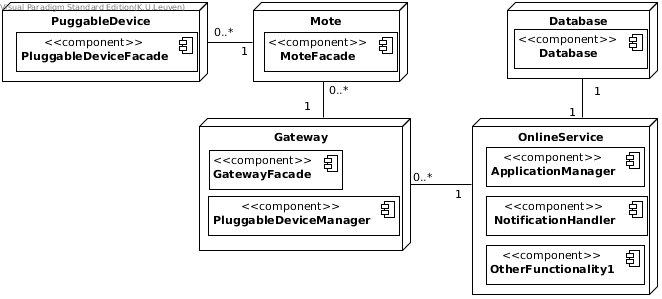
\includegraphics[width=1.00\textwidth]{deployment-diagram-1}
        	\caption{Deployment diagram of this decomposition.}\label{fig:it1-depl_main}
        \end{figure}


\subsection{Interfaces for child modules}\label{add1-interfaces}
    This section describes the interfaces assigned to the components defined
    in the section above. Per interface, we list its methods by means of its
    syntax. The data types used in these interfaces are defined in the following section. \\

    \noindent Each method shows which (part of a) quality attribute or use case caused
    a need for the method. However, this does not mean that a method is
    only to be used to satisfy that quality  attribute or use case, it could
    be used for other causes not yet mentioned here.

    \subsubsection{ApplicationManager}
        \begin{itemize}
            \item ForwardData
            \begin{itemize}
                \item \texttt{void sendData(PluggableDeviceData data)}
                \begin{itemize}
                    \item Effect: Send pluggable device data to an application that wants to use it
                    \item Created for:
                \end{itemize}
            \end{itemize}

            \item AppMgmt
            \begin{itemize}
                \item \texttt{void deactivateApplicationInstance(int applicationInstanceID)}
                \begin{itemize}
                    \item Effect: Deactivates a running instance of an application.
                    \item Created for:
                \end{itemize}
                \item \texttt{void activateApplicationInstance(int applicationInstanceID)}
                \begin{itemize}
                    \item Effect: Activates a new instance of an application.
                    \item Created for:
                \end{itemize}
            \end{itemize}
        \end{itemize}

    \subsubsection{Database}
        \begin{itemize}
            \item NotificationMgmt
            \begin{itemize}
                \item \texttt{int storeNotification(NotificationData data)}
                \begin{itemize}
                    \item Effect: Stores a new notification entry in the database. Returns the id of the new notification.
                    \item Created for:
                \end{itemize}
                \item \texttt{void updateNotification(NotificationData data)}
                \begin{itemize}
                    \item Effect: Updates an existing notification (e.g. change status to "sent").
                    \item Created for:
                \end{itemize}
                \item \texttt{int lookupNotificationChannelForUser(int userID)}
                \begin{itemize}
                    \item Effect: Returns the type of communication channel a user prefers.
                                  Different communication channels are mapped to integers.
                    \item Created for:
                \end{itemize}
            \end{itemize}

            \item AppDataMgmt
            \begin{itemize}
                \item \texttt{void updateApplication(ApplicationData data)}
                \begin{itemize}
                    \item Effect: Updates an application in the database (e.g. change state to 'inactive').
                    \item Created for:
                \end{itemize}
                \item \texttt{void updateSubscription(SubscriptionData data)}
                \begin{itemize}
                    \item Effect: Updates a subscription in the database (e.g. change state to 'disabled').
                    \item Created for:
                \end{itemize}
            \end{itemize}
        \end{itemize}

    \subsubsection{GatewayFacade}
        \begin{itemize}
            \item MoteDataMgmt
            \begin{itemize}
                \item \texttt{void sendHeartbeat(int moteID, List<PluggableDeviceInfo> devices)}
                \begin{itemize}
                    \item Effect: Sends a heartbeat to a certain gateway with information about operational devices.
                    \item Created for:
                \end{itemize}
            \end{itemize}

            \item DeviceMgmt
            \begin{itemize}
                \item \texttt{List<DeviceInfo> getConnectedDevices()}
                \begin{itemize}
                    \item Effect: Describe the effect of calling this operation.
                    \item Created for:
                \end{itemize}
                \item \texttt{void timerExpired(int deviceID)}
                \begin{itemize}
                    \item Effect: Lets the gateway know that a timer for pluggable device or mote has expired.
                                  This will generate a notification for an infrastructure owner.
                    \item Created for:
                \end{itemize}
                \item \texttt{void deactivateApplicationInstance(int applicationInstanceID)}
                \begin{itemize}
                    \item Effect: Deactivates a certain application. This could happen when
                                  mandatory pluggable devices for the application are missing.
                    \item Created for:
                \end{itemize}
                \item \texttt{void reactivateApplicationInstance(int applicationInstanceID)}
                \begin{itemize}
                    \item Effect: Reactivate an application instance. This could happen
                                  automatically after a broken sensor has been replaced.
                    \item Created for:
                \end{itemize}
            \end{itemize}

            \item AppDeviceMgmt
            \begin{itemize}
                \item \texttt{bool areEssentialDevicesOperational(int applicationID)}
                \begin{itemize}
                    \item Effect: Returns true if all essential devices for the application
                                  with id "applicationID" are operational.
                    \item Created for:
                \end{itemize}
            \end{itemize}
        \end{itemize}

    \subsubsection{MoteFacade}
        \begin{itemize}
            \item PluggableDeviceDataMgmt
            \begin{itemize}
                \item \texttt{List<DeviceInfo> getConnectedDevices()}
                \begin{itemize}
                    \item Effect: Returns a list of information about devices that are connected to the mote.
                    \item Created for:
                \end{itemize}
            \end{itemize}
        \end{itemize}

    \subsubsection{NotificationHandler}
        \begin{itemize}
            \item Notify
            \begin{itemize}
                \item \texttt{void notify(int userID, String message)}
                \begin{itemize}
                    \item Effect: Describe the effect of calling this operation.
                    \item Created for:
                \end{itemize}
            \end{itemize}

            \item DeliveryMgmt
            \begin{itemize}
                \item \texttt{void sendAcknowledgement(int notificationID)}
                \begin{itemize}
                    \item Effect: Sends an acknowledgement to the system for a certain notification.
                    \item Created for:
                \end{itemize}
            \end{itemize}
        \end{itemize}

    \subsubsection{External notification delivery serivce}
        \begin{itemize}
            \item NotificationDeliveryMgmt
            \begin{itemize}
                \item \texttt{void notify(JSONObject data)}
                \begin{itemize}
                    \item Effect: Deliver a notification to an end user using a specific delivery service.
                    \item Created for:
                \end{itemize}
            \end{itemize}
        \end{itemize}

    \subsubsection{PluggableDeviceManager}
        \begin{itemize}
        	\item DeviceListMgmt
        	\begin{itemize}
        		\item \texttt{void sendHeartbeat(int moteID, List<PluggableDeviceInfo> devices)}
        		\begin{itemize}
        			\item Effect: Send a heartbeat from a mote to check/update timers for operational devices.
        			\item Created for:
        		\end{itemize}
        		\item \texttt{bool areEssentialDevicesOperational(int applicationID)}
        		\begin{itemize}
        			\item Effect: Returns true if all essential devices for the application
                                  with id "applicationID" are operational.
        			\item Created for:
        		\end{itemize}
        	\end{itemize}
        \end{itemize}


\subsection{Data type definitions}
    This section defines the data types used in the interface descriptions above.

    \paragraph{PluggableDeviceData}
              contains data from a pluggable device at a certain point in time
              (value, type, date) (e.g. a sensor reading, an actuator status)
    \paragraph{PluggableDeviceSettings}
              contains settings for a pluggable device (power status,
              data update rate, ...)
    \paragraph{PluggableDeviceInfo}
              contains information about a pluggable device (device id,
              power status, data update rate, ...)
    \paragraph{NotificationData}
              contains data about a notification (message text, recipient,
              communication channel, date, status, source, ...).
    \paragraph{ApplicationData}
              contains data about an application instance (instance id, running status, ...)
    \paragraph{SubscriptionData}
              contains data about a subscription (subscription id, subscription status,
              subscription period, ...).


\subsection{Verify and refine}
    \noindent The selected architectural drivers have been handled completely
    in this decomposition.
    This section describes per component which (parts of) the remaining
    requirements it is responsible for. If requirements are split in
    multiple parts, this is indicated by the addition of a letter
    (or number, depending on the structure of the requirement) after their title.

    \paragraph{ApplicationManager}
        \begin{itemize}
            \item \emph{Av2}: Application failure \\
                   Prevention: a, b \\
                   Detection: a, b, c \\
                   Resolution: a, b, c
           \item \emph{P1}: Large number of users: c
           \item \emph{M1}: Integrate new sensor or actuator manufacturer: 1.c, 2.a
           \item \emph{M2}: Big data analytics on pluggable data and/or application usage data: d, e
           \item \emph{U1}: Application updates: a, b, c, d
           \item \emph{U2}: Easy Installation: e
           \item \emph{UC12}: Perform actuation command
           \item \emph{UC17}: Activate an application: 3, 4
        \end{itemize}

    \paragraph{Database}
        \begin{itemize}
          	\item None
        \end{itemize}

    \paragraph{GatewayFacade}
        \begin{itemize}
            \item \emph{Av1}: Communication between SIoTIP gateway and Online Service \\
                               Resolution: b, c, d
            \item \emph{M1}: Integrate new sensor or actuator manufacturer: 1.a, 2.b
            \item \emph{U2}: Easy Installation: a, c, d
            \item \emph{UC11}: Send pluggable device data: 1
        \end{itemize}

    \paragraph{MoteFacade}
        \begin{itemize}
            \item \emph{M1}: Integrate new sensor or actuator manufacturer: 1.a, 2.b
            \item \emph{U2}: Easy Installation: b, c, d
            \item \emph{UC04}: Install mote: 1, 2
            \item \emph{UC05}: Uninstall mote: 1
            \item \emph{UC06}: Insert a pluggable device into a mote: 2
            \item \emph{UC07}: Remove a pluggable device from its mote: 2
            \item \emph{UC11}: Send pluggable device data: 1
        \end{itemize}

    \paragraph{NotificationHandler}
        \begin{itemize}
            \item \emph{UC16}: Consult notification message: 5
            \item \emph{UC17}: Activate an application: 5, 6
        \end{itemize}

    \paragraph{OtherFunctionality1}
        \begin{itemize}
            \item \emph{Av1}: Communication between SIoTIP gateway and Online Service \\
                               Detection: a, b, c, d
                               Resolution: a
           	\item \emph{P1}: Large number of users: a
            \item \emph{P2}: Requests to the pluggable data database
            \item \emph{M1}: Integrate new sensor or actuator manufacturer: 1.d
            \item \emph{M2}: Big data analytics on pluggable data and/or application usage data: a
            \item \emph{U2}: Easy Installation: e
            \item \emph{UC01}: Register a customer organisation
            \item \emph{UC02}: Register an end-user
            \item \emph{UC03}: Unregister an end user
            \item \emph{UC04}: Install mote: 3
            \item \emph{UC05}: Uninstall mote: 2.b
            \item \emph{UC06}: Insert a pluggable device into a mote: 3: topology part; alternative 3a.1.b
            \item \emph{UC07}: Remove a pluggable device from its mote: 3.b
            \item \emph{UC08}: Initialise a pluggable device: 1, 2, 4
            \item \emph{UC09}: Configure pluggable device access rights
            \item \emph{UC10}: Consult and configure the topology
            \item \emph{UC11}: Send pluggable device data: 3
            \item \emph{UC13}: Configure pluggable device
            \item \emph{UC16}: Consult notification message: 1, 2, 3, 4
            \item \emph{UC17}: Activate an application: 1, 2
            \item \emph{UC19}: Subscribe to application
            \item \emph{UC20}: Unsubscribe from application
            \item \emph{UC21}: Send invoice
            \item \emph{UC22}: Upload an application
            \item \emph{UC23}: Consult application statistics
            \item \emph{UC24}: Consult historical data
            \item \emph{UC25}: Access topology and available devices
            \item \emph{UC26}: Send application command or message to external front-end
            \item \emph{UC27}: Receive application command or message to external front-end
            \item \emph{UC28}: Log in
            \item \emph{UC29}: Log out
        \end{itemize}

    \paragraph{PluggableDeviceFacade}
        \begin{itemize}
        	\item \emph{U2}: Easy Installation: d
        \end{itemize}

    \paragraph{PluggableDeviceManager}
        \begin{itemize}
            \item \emph{U2}: Easy Installation: c, d
            \item \emph{UC04}: Install mote: 4
            \item \emph{UC05}: Uninstall mote: 2
            \item \emph{UC06}: Insert a pluggable device into a mote: 3: uninitialised part; alternative 3a.1 3a.2 3a.4; 4
            \item \emph{UC07}: Remove a pluggable device from its mote: 3.a, 3.c
            \item \emph{UC08}: Initialise a pluggable device: 3
            \item \emph{UC11}: Send pluggable device data: 2, 3a
        \end{itemize}
